\chapter{Requirements specification}

The requirements for the product are prioritized using the MoSCoW method. Using this, the requirements for the product are divided into four sections, where the most important elements are given the highest priority. \textbf{Must} are the requirements that are an absolute necessity for the product. \textbf{Should} are the requirements that are also of high priority, but not quite mandatory. \textbf{Could} are requirements which may be met, if the time and other constraints of the project allow for it. \textbf{Won't} are the requirements the product will not meet, but could be developed at a later point in its lifetime.  

\noindent The following priorities have been chosen for this project:
\begin{itemize}
	\item[\textbf{Must}]
		\begin{itemize}
			\item Navigate waypoints from user input
			\item Be compatible with NMEA protocol GPS input
			\item Use GPS for localization
			\item Implement a PID control loop
		\end{itemize}
	\item[\textbf{Should}]
		\begin{itemize}
			\item Control thrusters in two-thruster catamaran
			\item Use a graphical user interface for user interaction
			\item Be able to change the PID parameters
		\end{itemize}
	\item[\textbf{Could}] 
		\begin{itemize}
			\item Control wheel in outboard motor on boat
			\item Be generic enough to use with other engine types
		\end{itemize}
	\item[\textbf{Won't}]
		\begin{itemize}
			\item Use pylogon-coverage for a specified area
			\item Avoid obstacles
		\end{itemize}
\end{itemize}

\section{Mockups}
To get a better understanding of what the system would require, some user interface mockups were created. 
The first of which, describe how there should be the ability to edit and change different parameters of the system, on figure~\ref{fig:mockup:edit_param}, it is seen how a profile 1 contains parameters for a PID. There is also the ability to create new profiles and change which on is the currently active one.

To describe a collection a parameters and to be able to switch the active one, there is a need for a term like a parameter profile.
This parameter profile is just a collection of parameters, and a name. It makes it easy to save different parameters and easily switch between them.

\begin{figure}[H]
	\centering
	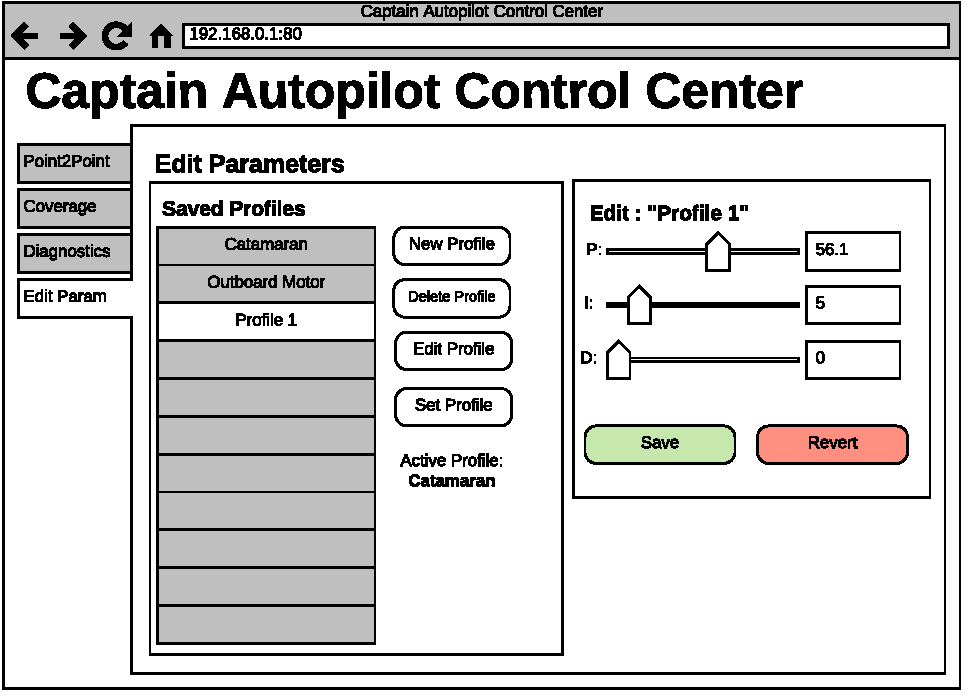
\includegraphics[width=1\linewidth]{Images/Requirements_specification/UI_Mockup_Edit_param.pdf}
	\caption{Mockup for Edit parameter menu}
	\label{fig:mockup:edit_param}
\end{figure}

The mockup in figure~\ref{fig:mockup:p2p} is describing how the user may define a waypoint for the boat to navigate. There is the ability of entering the coordinates by hand or by pressing the map. Also this page of the system allows the user to tell the ship to calculate a path with which to follow. An estimated time of arrival is also displayed.

\begin{figure}[H]
	\centering
	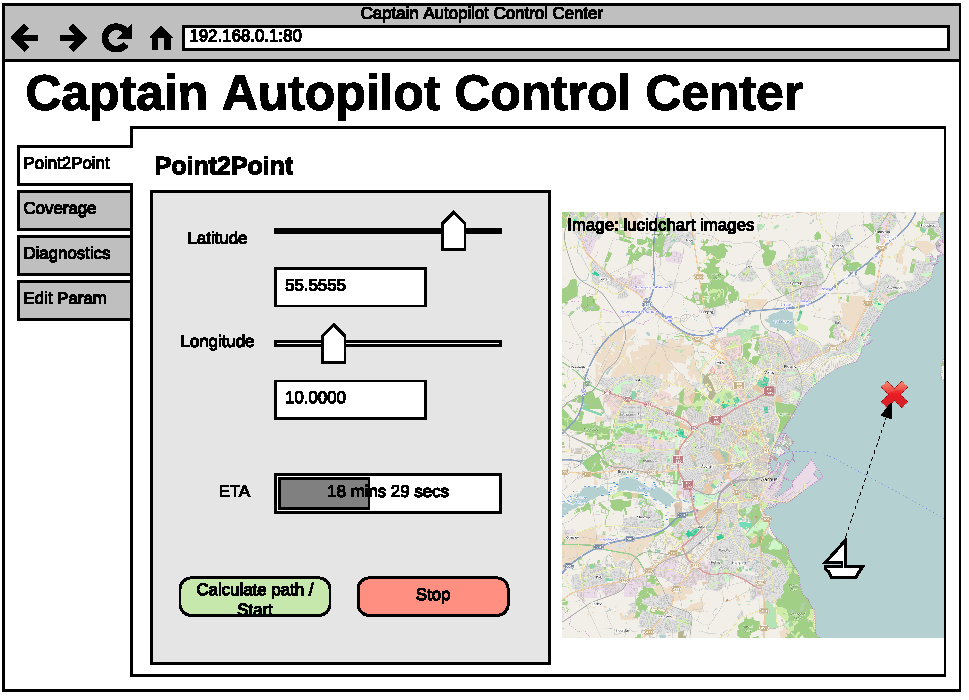
\includegraphics[width=1\linewidth]{Images/Requirements_specification/UI_Mockup_Point_to_point.pdf}
	\caption{Mockup for Point to point menu}
	\label{fig:mockup:p2p}
\end{figure}

There is also a mockup that describes how the user should define a rectangle to cover, seen in figure~\ref{fig:mockup:coverage}. like to the point to point menu mockup, there is a way to enter coordinates of the rectangle manually or by pressing the map. In every other regard this menu is just like the point to point menu.

\begin{figure}[H]
	\centering
	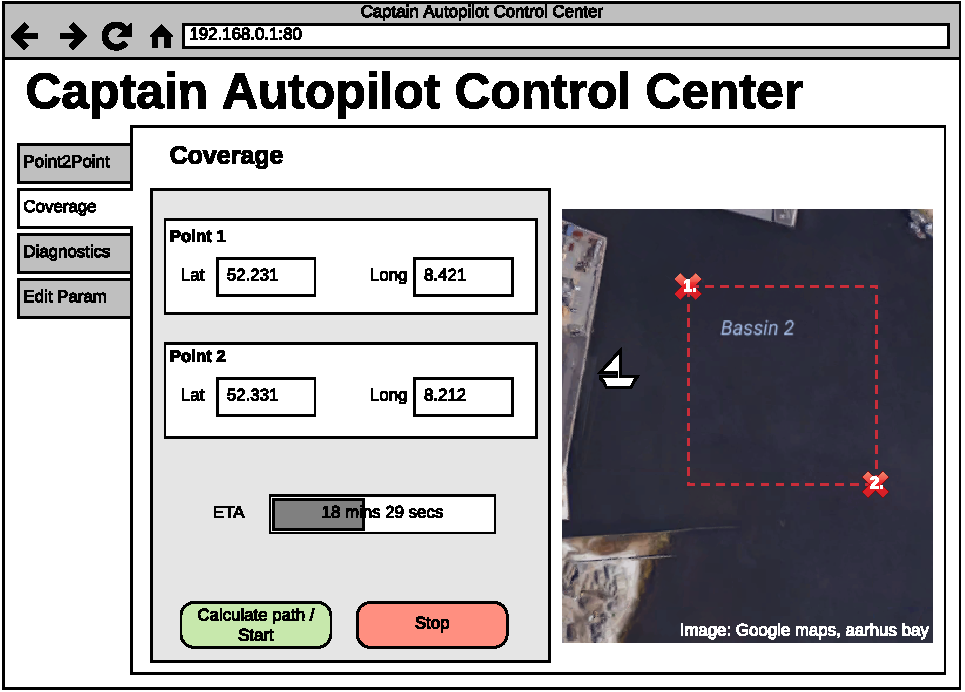
\includegraphics[width=1\linewidth]{Images/Requirements_specification/UI_Mockup_Coverage.pdf}
	\caption{Mockup for Coverage menu}
	\label{fig:mockup:coverage}
\end{figure}

Lastly there is a menu describe by the mockup on figure~\ref{fig:mockup:diagnostics} that show how the user of the system might see diagnostics data about the boat at any given time. The idea is that the boxes of information are interchangeable so if more information is required in the future is is easy to adapt the user interface.

\begin{figure}[H]
	\centering
	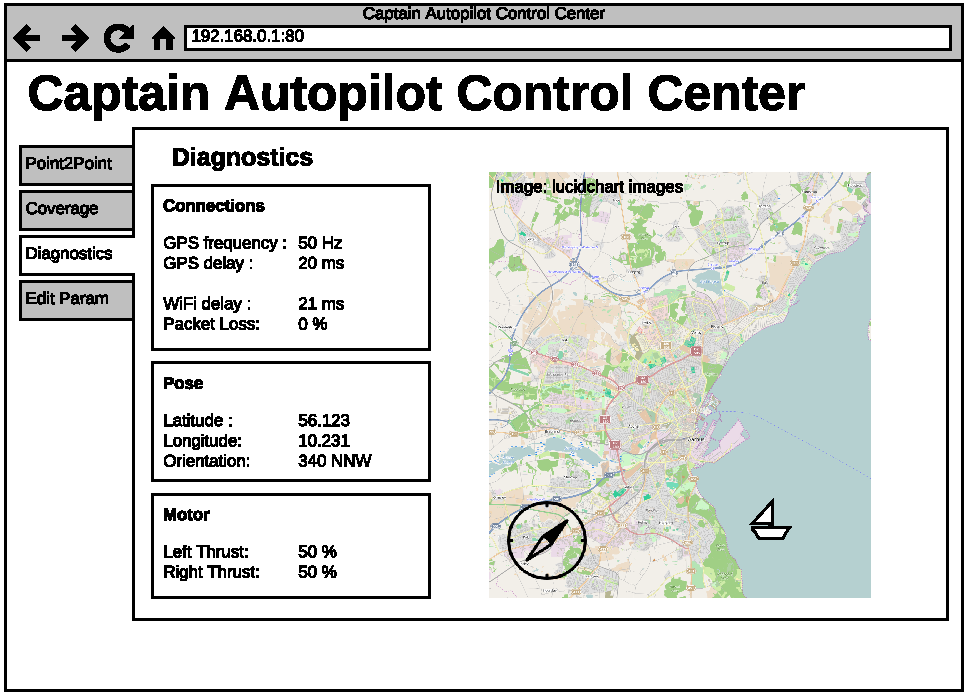
\includegraphics[width=1\linewidth]{Images/Requirements_specification/UI_Mockup_Diagnostics.pdf}
	\caption{Mockup for Diagnostics menu}
	\label{fig:mockup:diagnostics}
\end{figure}


The following two diagrams specify the actor context to the system, and the use cases for the system.

\section{Actors}
The following section describes the system's actors. Every actor has a type and a short description of its function and impact on the system. On figure~\ref{fig:actor} the actor context diagram is described. Actors on the left are primary actors, and on the right they are secondary actors.

\begin{figure}[H]
	\centering
	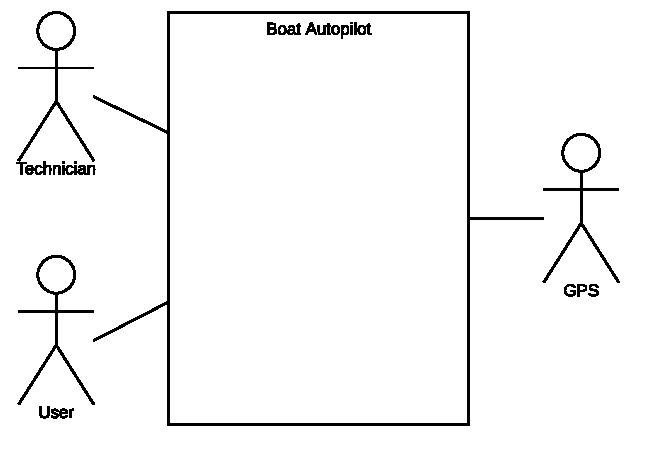
\includegraphics{Images/Requirements_specification/Actor_context_diagram}
	\caption{Actor context diagram}
	\label{fig:actor}
\end{figure}

\begin{framed}
	\subsection{Actor: Technician}
	\subsubsection*{Type:}
	Primary
	
	\subsubsection*{Description:}
	A technician with knowledge of the system. This actor triggers the use case "Specify parameters".
	
\end{framed}

\begin{framed}
	\subsection{Actor: User}
		\subsubsection*{Type:}
			Primary
	
		\subsubsection*{Description:}
			The user, or customer. This actor triggers the use case "Specify waypoints".
\end{framed}

\begin{framed}
	\subsection{Actor: GPS}
		\subsubsection*{Type:}
			Secondary
	
		\subsubsection*{Description:}
			The global positioning system. This actor assists in carrying out the use case "Navigate waypoints".
	
\end{framed}

\section{Fully dressed Use cases }
Use cases are used to describe the intended use of a system. When a system has a user interface, use cases make a lot of sense since for every action a user or actor has there should be some feedback of some kind. To get an overview of all the use cases a use case diagram can be created, it shows all primary and secondary actors of a system, an also which use cases they are involved in, as well as which they initiate, this is show with an arrow on figure~\ref{fig:usecasediagram}.

For each use case there is defined a goal, and a way to get to that goal, via the main scenario. There can be defined some prerequisites, that must be how the use case defines for the user to get the expected result. Also there might be extensions or exceptions that deviate from the main scenario. They also describe what actors are involved and what their role is. If a use case uses another use case there can be found a reference.

\begin{figure}[H]
	\centering
	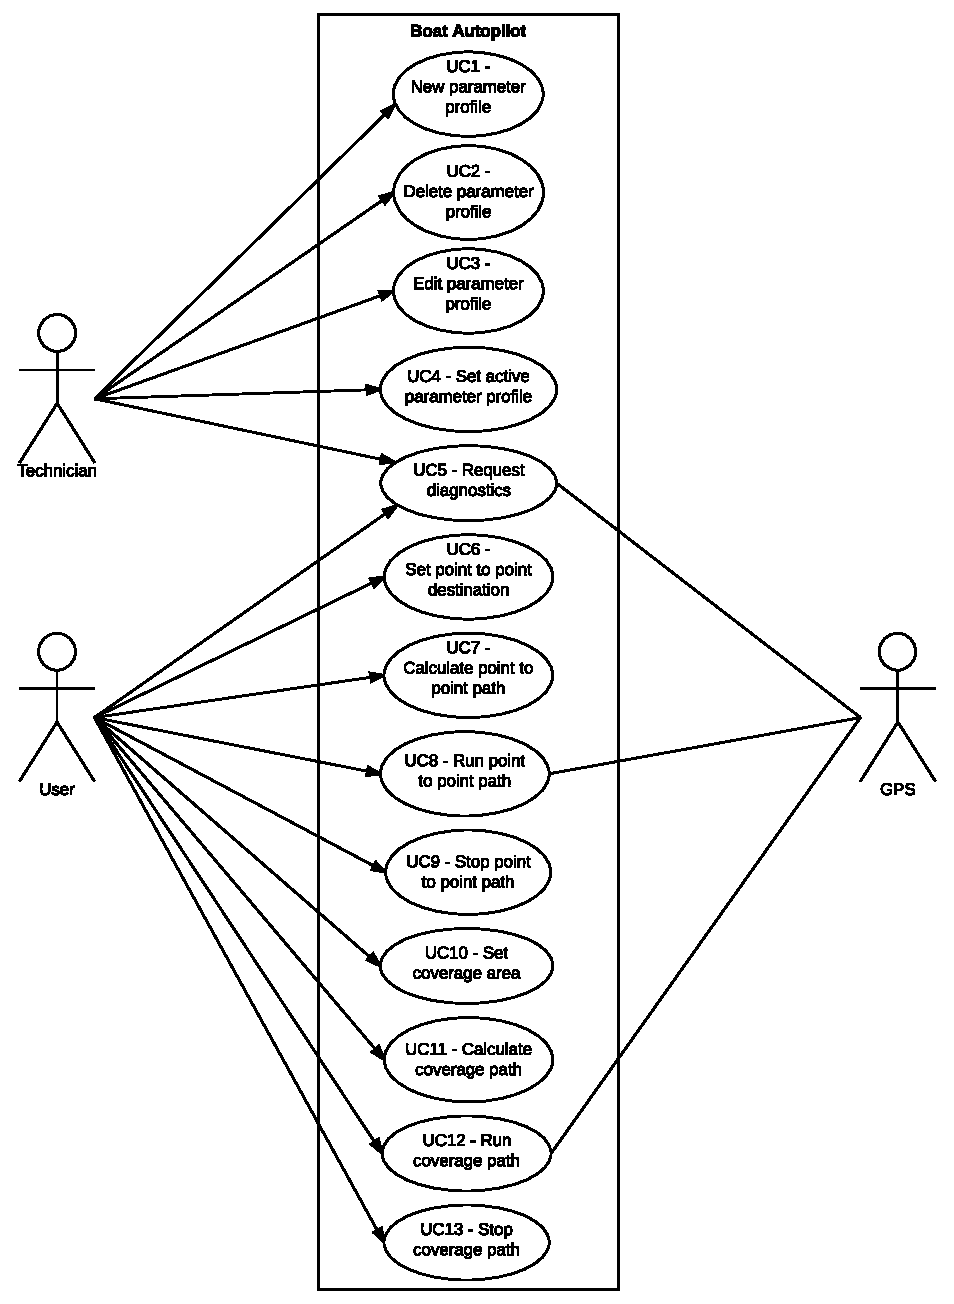
\includegraphics[width=0.9\linewidth]{Images/Requirements_specification/Usecase_diagram}
	\caption{Use case diagram}
	\label{fig:usecasediagram}
\end{figure}


\begin{framed}
\subsection{Use case 1 - New parameter profile}
\subsubsection*{Goal:}
To create a new parameter profile for the controller

\subsubsection*{Initialization:}
Technician

\subsubsection*{Actors:}
Technician (primary)

\subsubsection*{References:}
None

\subsubsection*{Simultaneous occurrences:}
One

\subsubsection*{Prerequisite:}
"Edit parameter" menu is opened in user interface

\subsubsection*{Result:}
A new parameter profile has been created.

\subsubsection*{Main scenario:}
\begin{enumerate}
	\item The technician selects "New" button.
	\item A new parameter profile is added to the list of parameter profiles, all parameters are set to default values.
	\item The selected parameter profile values are displayed on the user interface
\end{enumerate}	
\end{framed}

\begin{framed}
	\subsection{Use case 2 - Delete parameter profile}
	\subsubsection*{Goal:}
	To delete a parameter profile for the controller
	
	\subsubsection*{Initialization:}
	Technician
	
	\subsubsection*{Actors:}
	Technician (primary)
	
	\subsubsection*{References:}
	None
	
	\subsubsection*{Simultaneous occurrences:}
	One
	
	\subsubsection*{Prerequisite:}
	\begin{itemize}
		\item "Edit parameter" menu is opened in user interface
		\item A parameter profile must exist.
	\end{itemize}
	
	\subsubsection*{Result:}
	A parameter profile has been deleted
	
	\subsubsection*{Main scenario:}
	\begin{enumerate}
		\item The technician selects a desired parameter profile to delete
		\item The technician selects "Delete" button.
		\item The selected profile is deleted from the list of parameter profiles. [Extension 1]
	\end{enumerate}	
	
	\subsubsection*{Extension 1: Active profile deleted}
		\begin{enumerate}
			\item If the active profile is deleted, no active profile is set.
		\end{enumerate}
\end{framed}



\begin{framed}
\subsection{Use case 3 - Edit parameter profile}
\subsubsection*{Goal:}
To edit an existing parameter profile 

\subsubsection*{Initialization:}
Technician

\subsubsection*{Actors:}
Technician (primary)

\subsubsection*{References:}
None

\subsubsection*{Simultaneous occurrences:}
One

\subsubsection*{Prerequisite:}
\begin{itemize}
	\item "Edit parameter" menu is opened in user interface
	\item A parameter profile must exist.
\end{itemize}


\subsubsection*{Result:}
The parameter profile has been edited

\subsubsection*{Main scenario:}
\begin{enumerate}
	\item The technician selects a desired parameter profile to edit
	\item Then the technician selects "Edit"
	\item The selected parameter profile values are displayed on the user interface
	\item The technician edits the parameter values of the profile
	\item The technician selects "Save" [Extension 1]
	\item The old parameter profile is overwritten with the new values.
\end{enumerate}	

\subsubsection*{Extension 1: Revert}
	\begin{enumerate}
		\item The technician selects "Revert"
		\item The old parameter profile is not overwritten. The old values are kept
		\item The user interface displays the old values
	\end{enumerate}
\end{framed}

\begin{framed}
	\subsection{Use case 4 - Set active parameter profile}
	\subsubsection*{Goal:}
	To set a parameter profile as active.
	
	\subsubsection*{Initialization:}
	Technician
	
	\subsubsection*{Actors:}
	Technician (primary)
	
	\subsubsection*{References:}
	None
	
	\subsubsection*{Simultaneous occurrences:}
	One
	
	\subsubsection*{Prerequisite:}
	\begin{itemize}
		\item "Edit parameter" menu is opened in user interface
		\item A parameter profile must exist.
	\end{itemize}

	\subsubsection*{Result:}
	The parameter profile has been set as active
	
	\subsubsection*{Main scenario:}
	\begin{enumerate}
		\item The technician selects a desired parameter profile to activate
		\item The technician then selects "Activate"
		\item The selected parameter profile has been set as active.
		\item The name of the active profile is displayed on the user interface.
		\item The boat parameters are updated with the newly activated parameter profile values.
	\end{enumerate}
\end{framed}

\begin{framed}
	\subsection{Use case 5 - Request diagnostics}
	\subsubsection*{Goal:}
	To display all diagnostics data
	
	\subsubsection*{Initialization:}
	Technician or user
	
	\subsubsection*{Actors:}
	\begin{itemize}
		\item Technician (primary)
		\item User (primary)
		\item GPS (secondary)
	\end{itemize}
	
	\subsubsection*{References:}
	None
	
	\subsubsection*{Simultaneous occurrences:}
	One
	
	\subsubsection*{Prerequisite:}
	None
	
	\subsubsection*{Result:}
	All diagnostics data are displayed on the user interface
	
	\subsubsection*{Main scenario:}
	\begin{enumerate}
		\item The primary actor selects the "Status" menu in the user interface.
		\item The diagnostics data is displayed on the user interface. 
	\end{enumerate}
\end{framed}



\begin{framed}
	\subsection{Use case 6 - Set point to point destination}
	\subsubsection*{Goal:}
	To set a point to point destination
	
	\subsubsection*{Initialization:}
	User
	
	\subsubsection*{Actors:}
	User (primary)
	
	\subsubsection*{References:}
	None
	
	\subsubsection*{Simultaneous occurrences:}
	One
	
	\subsubsection*{Prerequisite:}
	\begin{itemize}
		\item The user interface has an updated map
		\item The "Point to point" menu is opened in user interface
	\end{itemize}

	\subsubsection*{Result:}
	A destination has been defined.
	
	\subsubsection*{Main scenario:}
	\begin{enumerate}
		\item The user selects a desired position on the map.
		\item \label{uc4.2} The user interface displays the selected position on the map
		\item The user interface displays the selected position as coordinates
	\end{enumerate}	

	\subsubsection*{Alternate flow 1: Coordinate input}
		\begin{enumerate}
			\item The user inputs latitude and longitude in the user interface
			\item The main scenario is continued from step \ref{uc4.2}.
		\end{enumerate}
\end{framed}	

\begin{framed}
	\subsection{Use case 7 - Calculate point to point path}
	\subsubsection*{Goal:}
	A path to the destination has been calculated.
	
	\subsubsection*{Initialization:}
	User
	
	\subsubsection*{Actors:}
	User (primary)
	
	\subsubsection*{References:}
	None
	
	\subsubsection*{Simultaneous occurrences:}
	One 
	
	\subsubsection*{Prerequisite:}
	\begin{itemize}
		\item Use case 6 - Set point to point destination has been completed
		\item The user interface has an updated map
		\item The "Point to point" menu is opened in user interface
		\item The boat must not be running a navigation task.
	\end{itemize}
	
	\subsubsection*{Result:}
	A path to the destination has been calculated.
	
	\subsubsection*{Main scenario:}
	\begin{enumerate}
		\item The user selects "Calculate path" from the user interface.
		\item A path is calculated and displayed on the map. 
		\item The "Calculate path" option is changed to "Start"
	\end{enumerate}	
\end{framed}	


\begin{framed}
	\subsection{Use case 8 - Run point to point path}
	\subsubsection*{Goal:}
	The boat reaches the point to point destination
	
	\subsubsection*{Initialization:}
	User
	
	\subsubsection*{Actors:}
	User (primary)
	
	\subsubsection*{References:}
	Use case 7 - Calculate point to point path
	
	\subsubsection*{Simultaneous occurrences:}
	One 
	
	\subsubsection*{Prerequisite:}
	\begin{itemize}
		\item The user interface has an updated map
		\item The "Point to point" menu is opened in user interface
		\item Use case 7 - Calculate point to point path has been completed
		\item There must be an active parameter profile.
		\item The boat must not be running a navigation task.
	\end{itemize}
	
	\subsubsection*{Result:}
	The destination is reached
	
	\subsubsection*{Main scenario:}
	\begin{enumerate}
		\item The user selects "Start".
		\item The "Start" button on the user interface changes to read "Running...".
		\item The boat runs a control loop based on direction data from the calculated path.
		\item The position of the boat on the user interface map is continually updated using GPS.
		\item The ETE is continually calculated and displayed on the user interface.
		\item When the boat reaches its destination it stops.
		\item On the user interface the "Running..." button is replaced by the "Calculate path" button.
	\end{enumerate}	
\end{framed}	

\begin{framed}
	\subsection{Use case 9 - Stop point to point path}
	\subsubsection*{Goal:}
	The boat stops while running point to point navigation
	
	\subsubsection*{Initialization:}
	User
	
	\subsubsection*{Actors:}
	User (primary)
	
	\subsubsection*{References:}
	Use case 8 - Run point to point path
	
	\subsubsection*{Simultaneous occurrences:}
	One 
	
	\subsubsection*{Prerequisite:}
	\begin{itemize}
		\item The user interface has an updated map
		\item The "Point to point" menu is opened in user interface
		\item Use case 8 - Run point to point is running
		\item There must be an active parameter profile.
		
	\end{itemize}
	
	\subsubsection*{Result:}
	The boat has stopped
	
	\subsubsection*{Main scenario:}
	\begin{enumerate}
		\item The user selects "Stop".
		\item The "Running..." button changes to the "Calculate path" button.
		\item The boat turns off its motors and comes to a halt.
	\end{enumerate}	
\end{framed}	

\begin{framed}
	\subsection{Use case 10 - Set coverage area}
	\subsubsection*{Goal:}
	To specify an area to cover.
	
	\subsubsection*{Initialization:}
	User
	
	\subsubsection*{Actors:}
	User (primary)
	
	\subsubsection*{References:}
	None
	
	\subsubsection*{Simultaneous occurrences:}
	One
	
	\subsubsection*{Prerequisite:}
	\begin{itemize}
		\item The user interface has an updated map
		\item The "Coverage" menu is opened in user interface
	\end{itemize}
	
	\subsubsection*{Result:}
	A coverage area has been defined
	
	\subsubsection*{Main scenario:}
	\begin{enumerate}
		\item The user selects two positions on the map which encapsulates a rectangle. One of the points is labeled "1", this specifies the starting point of the coverage route, the other is labeled "2" indicating the endpoint.
		\item \label{uc10.2} The user interface displays the selected rectangle on the map, including the staring point "1" and endpoint "2".
		\item The user interface displays the selected points as coordinates.
	\end{enumerate}	
	
	\subsubsection*{Alternate flow 1: Coordinate inputs}
		\begin{enumerate}
			\item The user inputs latitude and longitude for each point "1" and "2" in the user interface.
			\item The main scenario is continued from \ref{uc10.2}
		\end{enumerate}
\end{framed}	

\begin{framed}
	\subsection{Use case 11 - Calculate coverage path}
	\subsubsection*{Goal:}
	To calculate a path that covers an area.
	
	\subsubsection*{Initialization:}
	User
	
	\subsubsection*{Actors:}
	User (primary)
	
	\subsubsection*{References:}
	Use case 10 - Set coverage area
	
	\subsubsection*{Simultaneous occurrences:}
	One 
	
	\subsubsection*{Prerequisite:}
	\begin{itemize}
		\item The user interface has an updated map
		\item The "Coverage" menu is opened in user interface.
		\item The area to cover must be defined.
		\item The boat must not be running a navigation task.
	\end{itemize}
	
	\subsubsection*{Result:}
	A path to the destination has been calculated.
	
	\subsubsection*{Main scenario:}
	\begin{enumerate}
		\item The user selects "Calculate path" from the user interface.
		\item A path is calculated and displayed on the map. 
		\item The "Calculate path" option is changed to "Start"
	\end{enumerate}	
\end{framed}	

\begin{framed}
	\subsection{Use case 12 - Run coverage path}
	\subsubsection*{Goal:}
	The boat completes its coverage path.
	
	\subsubsection*{Initialization:}
	User
	
	\subsubsection*{Actors:}
	User (primary)
	
	\subsubsection*{References:}
	Use case 11 - Calculate coverage path
	
	\subsubsection*{Simultaneous occurrences:}
	One 
	
	\subsubsection*{Prerequisite:}
	\begin{itemize}
		\item The user interface has an updated map
		\item The "Coverage" menu is opened in user interface
		\item Use case 11 - Calculate coverage path has been completed
		\item There must be an active parameter profile.
		\item The boat must not be running a navigation task.
	\end{itemize}
	
	\subsubsection*{Result:}
	The coverage path is completed.
	
	\subsubsection*{Main scenario:}
	\begin{enumerate}
		\item The user selects "Start".
		\item The "Start" button on the user interface changes to read "Running...".
		\item The boat runs a control loop based on direction data from the calculated coverage path.
		\item The position of the boat on the user interface map is continually updated using GPS.
		\item The ETE is continually calculated and displayed on the user interface.
		\item When the boat reaches its destination, it stops.
		\item On the user interface the "Running..." button is replaced by a "Calculate path" button.
	\end{enumerate}	
\end{framed}	

\begin{framed}
	\subsection{Use case 13 - Stop point to point path}
	\subsubsection*{Goal:}
	The boat stops while running coverage navigation
	
	\subsubsection*{Initialization:}
	User
	
	\subsubsection*{Actors:}
	User (primary)
	
	\subsubsection*{References:}
	Use case 12 - Run coverage path
	
	\subsubsection*{Simultaneous occurrences:}
	One 
	
	\subsubsection*{Prerequisite:}
	\begin{itemize}
		\item The user interface has an updated map
		\item The "Coverage" menu is opened in user interface
		\item Use case 12 - Run coverage path is running
		\item There must be an active parameter profile.
		
	\end{itemize}
	
	\subsubsection*{Result:}
	The boat has stopped
	
	\subsubsection*{Main scenario:}
	\begin{enumerate}
		\item The user selects stop.
		\item The "Running..." button changes to a "Calculate path" button.
		\item The boat turns off its motors and comes to a halt.
	\end{enumerate}	
\end{framed}	

%\section{Non-functional requirements}

%WAAS GPS
%Controller: Ethernet port, built-in WiFi





